\section{Introduction, Scope and Context}
\label{sec:introduction}

Knowledge workers spend a fifth of their time just searching for information \parencite{mckinsey2012}. Investment banking (IB) is more affected than most. Document preparation consumes half to three-quarters of a junior banker's week, and pitch books (PBs) account for a large portion of that time \parencite{cfi2025,wso2024}. When Goldman Sachs surveyed its first-year analysts in 2021, the average was 98 hours a week, with document preparation a major driver of burnout \parencite{bbc2021}. Yet most PBs look nearly identical. Change the company name and update the numbers, and you could reuse last month's deck. That repetition makes them good targets for automation (K1, K7).

IB firms advise companies on mergers, acquisitions, capital raising, and other financial transactions. PBs are the primary vehicle for communicating analysis to clients and internal stakeholders. Getting these documents right matters, but getting them done quickly matters too.

Firms have tried internal document libraries, formatting specialists, and automation tools. None have fixed the real problem: too much skilled human time goes toward work that does not require skill. \textcite{chaves2022} found that knowledge sharing in banking suffers from structural barriers and inadequate digital tools, with company knowledge locked in individual documents rather than shared systems.

\subsection{Analyst Time Allocation}

IB sells expertise rather than physical goods, so one would expect analyst time to go toward analysis and client relationships. Often it does not.

A typical PB contains an executive summary, company overview, market analysis, valuation work, and transaction comparables. These sections appear in nearly every deck. The data inside changes, but the shell around it rarely does.

Analyst tasks fall into two buckets. The first holds work that genuinely needs a trained banker: modelling, valuation, and client advisory. The second holds everything else: hunting down data, reformatting slides, and fixing fonts. Too many hours go into the second bucket.

The process follows a predictable pattern: dig through document archives for similar deals, pull financial data from Bloomberg and public filings, copy it into PowerPoint, reformat everything to match the firm's visual standards, then send it up for review. Senior bankers mark it up, and the cycle repeats until the document is ready. Every step has friction. Archive searches are slow, data entry is error-prone, and formatting is tedious.

Banks pay junior analysts well, so time on low-skill tasks is a poor return on that investment. \textcite{radhakrishna2024} found that well-designed knowledge management systems boosted productivity by 20 to 25 percent, with document production identified as a prime candidate for automation.

\textcite{mckinsey2012} found that knowledge workers spend 28\% of their workweek managing email and nearly 20\% searching for internal information. APQC research puts the figure higher: a quarter of all working time is lost to duplicated work and information retrieval \parencite{apqc2023}. Figure~\ref{fig:time-allocation} illustrates these drains. IB analysts likely fare worse given the document-intensive nature of the work.

\begin{figure}[H]
\centering
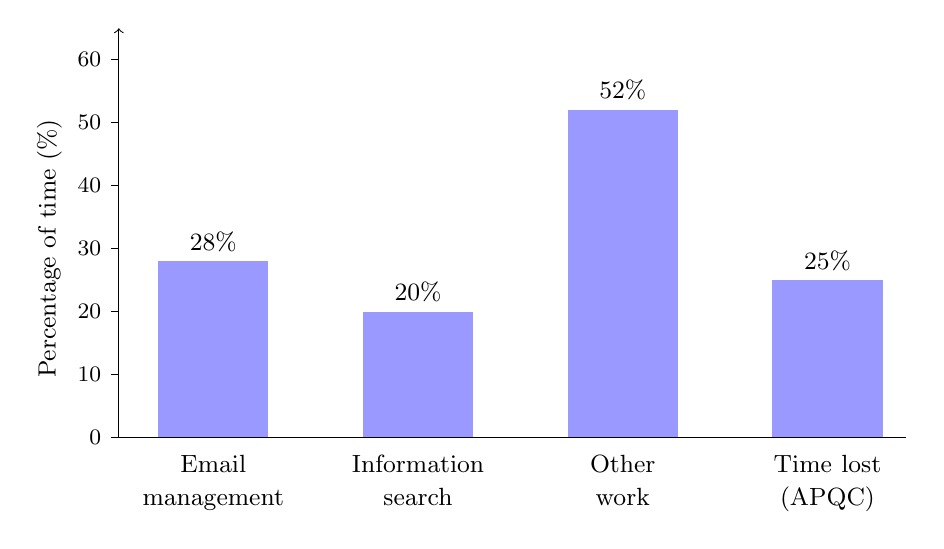
\begin{tikzpicture}
\pgfmathsetmacro{\barw}{1.4}   % bar width in cm
\pgfmathsetmacro{\gap}{2.6}    % centre-to-centre spacing
\pgfmathsetmacro{\scale}{0.08} % 1 percentage point = 0.08 cm
% Bars
\foreach \i/\val/\lab in {0/28/Email\\management, 1/20/Information\\search, 2/52/Other\\work, 3/25/Time lost\\(APQC)} {
    \pgfmathsetmacro{\x}{\i*\gap}
    \pgfmathsetmacro{\h}{\val*\scale}
    \fill[blue!40] (\x-\barw/2, 0) rectangle (\x+\barw/2, \h);
    \node[above] at (\x, \h) {\small \val\%};
    \node[below, text width=2cm, align=center] at (\x, -0.1) {\small \lab};
}
% Y axis
\draw[->] (-1.2, 0) -- (-1.2, 60*\scale+0.4);
\node[rotate=90, anchor=south] at (-1.8, 60*\scale/2) {\small Percentage of time (\%)};
% Y ticks
\foreach \val in {0, 10, 20, 30, 40, 50, 60} {
    \pgfmathsetmacro{\yy}{\val*\scale}
    \draw (-1.3, \yy) -- (-1.2, \yy);
    \node[left, font=\footnotesize] at (-1.3, \yy) {\val};
}
% X axis
\draw (-1.2, 0) -- (3*\gap+\barw/2+0.3, 0);
\end{tikzpicture}
\caption{Knowledge worker time allocation based on \textcite{mckinsey2012} and \textcite{apqc2023} research. The `other work' category represents the remaining time after email and search activities.}
\label{fig:time-allocation}
\end{figure}

In short, banks hire analysts for their analytical skills but spend a large share of their time on formatting and data entry. Existing tools have not solved this because they either miss IB visual standards or require too much manual work. Every hour on low-value tasks is an hour not spent on the analysis that sets one bank apart from another.

The competitive advantage is direct (K1). Banks that automate low-value work free their analysts to spend more time on client relationships and deal analysis. \textcite{dellacqua2023} found that consultants using AI completed 12.2\% more tasks at 40\% higher quality. If banks capture even half of that productivity gain on pitch book preparation, the impact compounds across hundreds of analysts and thousands of decks per year. The bank that gets a polished deck to the client a day earlier wins more mandates than the bank whose analysts are still reformatting slides at midnight.

\subsection{Problem Analysis}

\textcite{markus2001} defined knowledge reuse, and her framework fits PB production well. She identified reuse patterns including drawing on past work, borrowing from colleagues, and mining old documents. PB creation involves all of these. Three obstacles prevent effective reuse in practice.

The first obstacle is that too much time goes to low-value work. Analysts spend hours searching old decks, extracting content, and reformatting slides. None of that requires analytical thinking, yet it crowds out the work that does.

The second obstacle is that company knowledge tends to disappear. Researchers distinguish between tacit knowledge (in people's heads) and explicit knowledge (written down) \parencite{dalkir2011}. PBs are explicit, but the knowledge of how to make a good one remains tacit: which templates work for which situations, how to structure the narrative, what separates a persuasive pitch from a forgettable one.

The third obstacle is that onboarding takes longer than it should. Each bank has its own templates, data sources, and quality expectations. Junior analysts absorb these through trial and error, which is slow for them and a drain on the senior bankers who review their work.

These problems feed each other. Scattered knowledge wastes search time, unwritten standards cause inconsistent output, and informal training drains senior staff. A system that fixed even one of these would help.

\subsection{Gap Analysis}

Automated presentation tools have existed for years. Early versions converted text to slides using layout algorithms, but visual quality was poor \parencite{zheng2025}. Template-based systems fixed the visual problems but made everything rigid. PPTAgent \parencite{zheng2025} takes a different approach: it analyses reference presentations, extracts structural patterns, and applies them to new content. It beat older text-to-slide systems on both content and design quality in testing.

The limitation is that PPTAgent targets general-purpose presentations. IB PBs have financial tables, transaction comparables, and market charts that follow specific visual conventions. Getting the template wrong undermines credibility. Commercial tools like Beautiful.ai, Tome, and Gamma share this flaw: the output is generic, every slide needs rework, and none connect to financial data sources. IB PBs require both domain knowledge and visual precision, and no existing tool handles both.

Current systems either produce generic output that needs heavy cleanup, or they require large training datasets most banks lack. No existing tool connects slide generation to financial APIs. Data retrieval and document generation remain separate manual steps.

Agentic AI architectures offer a better fit \parencite{ibm2024}. Instead of one model doing everything in a single pass, the system breaks tasks into steps and uses the right tool for each one. \textcite{wang2024} surveyed LLM-based agents and found rapid progress. McKinsey \& Company estimates generative AI could deliver \$340 billion annually in banking \parencite{mckinsey2024}.

This project fills that gap (S1). The pipeline extracts layouts, colour palettes, and placeholder positions from a template using JSZip and xml2js for XML-level parsing, uses an LLM to plan content, then assembles slides matching the original style. The system uses an agentic orchestration pattern with specialised service components rather than a monolithic approach.

Table~\ref{tab:gap-objectives} maps each identified gap to the objective and success criterion that addresses it, so that no objective exists without a corresponding gap in existing work.

\begin{table}[H]
\centering
\begin{tabular}{|p{4.2cm}|l|p{4.5cm}|}
\hline
\textbf{Gap in Existing Work} & \textbf{Objective} & \textbf{Success Criterion} \\
\hline
No tool preserves exact template formatting & O1 & 90\%+ placeholder detection; exact colour extraction \\
\hline
Data retrieval and slide generation are separate manual steps & O2 & 100\% data accuracy against source APIs \\
\hline
No IB-specific content structuring & O3 & 3 PB types with consistent section ordering \\
\hline
Generic output that ignores corporate visual standards & O4 & Exact colour and font match against template \\
\hline
No measured evaluation of template-constrained generation & O5 & Full deck in under 5 minutes; template match above 85\% \\
\hline
\end{tabular}
\caption{Traceability from Research Gaps to Objectives and Success Criteria}
\label{tab:gap-objectives}
\end{table}

The approach differs from prior work in three ways. First, it inverts the typical generation order: the system starts with visual constraints extracted from the template and works backward to content, rather than generating content and hoping the formatting works. Second, it connects slide generation directly to financial data APIs, closing the gap between data retrieval and document creation. Third, it uses a service-oriented architecture where specialised components handle distinct parts of the task, making the system easier to test and modify independently.

\subsection{Business Case}

The financial case for automating pitch book production is straightforward. A junior IB analyst in London earns roughly \pounds 60,000 to 70,000 in base salary \parencite{glassdoor2025}. At 80 to 100 hours per week, the effective hourly cost is around \pounds 15 to 17 before overhead. Banks bill clients at significantly higher rates. If an analyst spends 15 hours per week on pitch book formatting and data entry, that is roughly \pounds 250 per week in salary alone going toward work that does not need analytical skill.

The system generates a first draft in under one minute. Manual creation of the same output takes 90 to 120 minutes. Even accounting for 20 to 30 minutes of human review and editing after generation, the net saving is roughly 60 to 90 minutes per deck. An analyst working on three to five decks per week saves three to seven hours, freeing that time for analysis, client work, or reduced overtime.

On the cost side, each generation request costs approximately \$0.03 in GPT-4o API fees. Hosting costs (Vercel, Render, Supabase) fall within free tiers at proof-of-concept scale. At production scale with 1,000 daily requests, monthly API costs would be roughly \$900, still far below the salary cost of the manual hours replaced.

The return on investment is clear even at small scale (K2). A team of ten analysts saving five hours per week each recovers 50 analyst-hours weekly. At a conservative internal cost of \pounds 15 per hour, that is \pounds 750 per week or roughly \pounds 39,000 per year in recovered capacity, against annual API costs under \pounds 10,000. The payback period is under four months.

\subsection{Aims and Objectives}

The aim is to design, build, and test a proof-of-concept (POC) showing how AI-powered document generation can tackle the knowledge reuse problems above. The system must respect company templates throughout. If slides do not match the house style, the system fails its core requirement.

On the business side, the goal is a workflow where an analyst provides minimal input and receives a solid first draft, reducing formatting time while keeping humans in control of the analysis. Target users are junior analysts.

On the learning side, the project explores how to connect LLM orchestration with programmatic document generation: agentic architectures, template pattern extraction, and end-to-end AI pipeline design. Human-in-the-loop (HITL) design is central, since AI tools in regulated industries need to support professional judgement rather than replace it. The constraint-first approach (extracting visual and structural rules before generating content) is the main technical contribution. The same idea would work wherever generated output must match precise formatting: legal briefs, consulting reports, or regulatory filings.

Five objectives structure the work:

\begin{enumerate}
    \item Build a template analysis component that takes a reference PowerPoint file and extracts its layout structures, colour palettes, font specifications, and placeholder positions. Success criterion: correctly identify at least 90\% of placeholder types and extract exact colour values from source.
    \item Build an agentic data retrieval layer that automatically pulls company financials, market data, and regulatory filings from Yahoo Finance and SEC EDGAR (the US Securities and Exchange Commission's public database of company filings). Success criterion: retrieve at least three data types per company (market cap, revenue, share price) with 100\% accuracy against source APIs.
    \item Build an LLM-powered content planning module that produces structured slide specifications adapted to different PB types while keeping the overall narrative coherent. Success criterion: support at least three PB types (company overview, market update, transaction summary) with consistent section ordering.
    \item Build a slide assembly component that takes the content plan and template patterns and produces a PowerPoint file meeting formatting standards. Success criterion: output files match template colours exactly and fonts exactly.
    \item Evaluate the system by measuring generation speed, template matching, and content quality. Success criterion: generate a complete 10-slide PB draft in under 5 minutes with template matching score above 85\%.
\end{enumerate}

\subsection{Scope and Success Criteria}

The POC takes user input (company, transaction type, dates, reference template, PB type) and produces a formatted PowerPoint. Target PB types are company overviews, market updates, and transaction summaries. Full valuation presentations are out of scope.

Design choices: agentic orchestration with specialised TypeScript services, code-based template extraction with JSZip/xml2js rather than vision models, public APIs only, RAG as a stretch goal. Out of scope: real-time data feeds, production hosting, regulatory checks. Practical limits: one academic term, standard hardware, student API budget.

Several assumptions constrain the scope. Templates are assumed to be well-formed Office Open XML archives following standard PowerPoint conventions; templates with corrupted XML or non-standard packaging are not supported. All financial data comes from public sources (Yahoo Finance, SEC EDGAR), so coverage is limited to publicly listed companies with available filings. Content is generated in English only. The system assumes that users have access to desktop PowerPoint on Windows or macOS, since the add-in relies on Office.js APIs that PowerPoint for the web does not fully support. The LLM (GPT-4o) is accessed via OpenAI's API under their standard usage terms, which prohibit using outputs to train competing models but impose no restrictions relevant to document generation.

Success criteria:

\begin{itemize}
    \item Generate complete PB draft within five minutes
    \item Match reference template formatting
    \item Accurate financial data from source APIs
    \item Content structure following IB conventions, verified against precedent examples
\end{itemize}

One principle runs through all of this: HITL design. The system produces drafts for human review, not finished products. AI can handle the mechanical work; the analytical judgement stays with the banker.
